\documentclass[a4paper,10pt]{article}
\usepackage[utf8]{inputenc}
\usepackage[T1]{fontenc}	
\usepackage[italian]{babel}

\usepackage{amsmath}
\usepackage{amsfonts}
\usepackage{amssymb}
\usepackage{graphicx}

\usepackage[left=2cm,right=2cm,top=2cm,bottom=2cm]{geometry}
\geometry{a4paper}

\usepackage{booktabs}
\usepackage{verbatim}
\usepackage{subfig}
\usepackage[dvipsnames]{xcolor}  %colori
\usepackage[colorlinks=true, linkcolor=black, urlcolor=blue, citecolor=darkgray, filecolor=darkgray]{hyperref}   %per gli hyperlink

\usepackage[cdot, thickqspace, squaren]{SIunits}
\usepackage{float}

% macro
\def\code#1{\texttt{#1}}

\title{Esperienza porta Not} % bha il titolo andrebbe migliorato
\author{Gruppo BL \\ Candido Alessandro, Luzio Andrea, Mazziotti Fabrizio}

\begin{document}

\maketitle

%\begin{abstract}
%Lo scopo di questa esperienza è di
%\end{abstract}



\section{Scopo e Strumentazione}
Lo scopo dell'esperienza è Misurare le caratteristiche statiche e dinamiche delle porte NOT contenute nell’integrato \code{SN74LS04} (HEX Inverter).

La strumentazione è quella solitamente presente sul banco di lavoro, e inoltre si è usato:
\begin{itemize}
	\item \code{IC SN74LS04};
	\begin{itemize}
		\item Trimmer da $2~$K e $100~$K;
	\end{itemize}
	\item Arduino Nano; 
	\begin{itemize}
		\item \code{IC SN74LS244} octal buffer/driver; 
		\item Trimmer da $10~$K;
	\end{itemize}
\end{itemize}

%\subsection{Errori sistematici}
%
%\begin{itemize}
%
% \item Oscilloscopio digitale Tektronix TDS 1012. \newline
% 		Lo strumento è affetto da erorre sistematico del 3 \% sulle scale di tensione utilizzate, e di 100 ppm sulle scale di tempo utilizzate.
% \item Tester digitale Konig KDM-350CTF. \newline con errore sistematico del 0.5 \% sulle scale di tensione, 0.8\% su tutte le scale di resistenza utilizzate. Per quanto riguarda l'errore sistematico relativo alle capacità è del 4\%.
%
%\end{itemize}

\section{Caratteristiche statiche}

\subsection{Misura delle tensioni di operazione}

\begin{figure}[H]
	\centering
	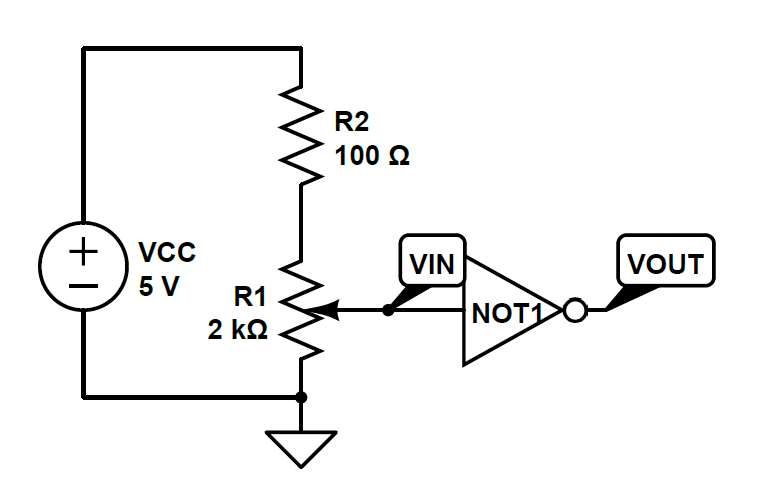
\includegraphics[width=0.7\textwidth]{../grafici/NOTin.png}
	\caption{}
	\label{fig:NOTin}
\end{figure}
Per misurare la caratteristica $V_{in}-V_{out}$ della porta not presa in esame si è montato il circuito come in \ref{fig:NOTin}. Sono stati misurati i valori delle resistenze $R_2$ e il massimo di $R_1$e, sebbene il funzionamento del circuito sia indipendente dai valori precisi essi, sono tabulati in tabella \ref{Res1}.

\begin{table}[H]
	\centering
	\begin{tabular}{c|c}
		\hline
		$R_1 = \unit{1.979 \pm 0.017}{\kilo\ohm}$ & $R_2 = \unit{99.7 \pm 1.1}{\ohm}$\\
		\hline
	\end{tabular}
	\caption{}
	\label{Res1}
\end{table}

\'E dunque stata presa la tensione di ingresso (con il multimetro digitale) e la tensione di uscita (con l'oscilloscopio) per diversi valori della resistenza $R_1$.I dati raccolti sono riassunti in \ref{fig:VinVout}.


\begin{figure}[H]
	\centering
	\includegraphics[width=0.7\textwidth]{../grafici/VinVout.pdf}
	\caption{Dati sperimentali relativi alle tensioni in uscita in funzione delle tensioni in ingresso. La tensione di alimentazione è $ \unit{4.95 \pm 0.03}{\volt}$}
	\label{fig:VinVout}
\end{figure}

Questo grafico è da commentare. Fino a una certa tensione in ingresso $V_{IH}$ l'uscita è chiaramente HIGH. Questa tensione è osservabile dal grafico ed è collocabile tra i 0.80 e i 0.90 V. Se ne da dunque una stima di $0.85 \pm 0.05 V$. Come errore si è preferito scegliere la semidispersione in quanto "valore di riferimento". 
Aumentando ancora la tensione di ingresso si ha dunque un crollo della tensione di uscita che si stabilizza al suo valore finale verso i 1.06-1.08 v. Al di sopra di questa seconda tensione l'output è stabilmente LOW. Si è dunque stimato il valore di $V_{IL}=1.07 \pm 0.01 V$. 


Si può capire meglio che cosa succede osservando il comportamento del circuito con l'oscilloscopio. Si osserva in pratica che l'output, per valori di tensione vicini alla discontinuità vista nel grafico, è rumorosissimo. Questo è ovvio se si considera quanto può variare in quella regione l'output a causa di anche piccoli rumori dell'input\footnote{ Rumore che possono anche essere interni alla porta.}.
In pratica il marcato rumore è presente tra $1.03 V$ e $1.01 V$.


Gli stessi dati sono stati presi sostituendo il partitore di ingresso con l'uscita del generatore di tensione settato per generare una rampa triangolare.
Sono stati ottenuti i dati rappresentati nelle figure \ref{fig:oscRaw} e \ref{fig:osc}.

\begin{figure}[H]
	\centering
	\includegraphics[width=0.7\textwidth]{../grafici/oscRaw.pdf}
	\caption{I due canali ottenuti direttamente dall'oscilloscopio. La tensione di alimentazione della porta è sempre $ \unit{4.95 \pm 0.03}{\volt}$}
	\label{fig:oscRaw}
\end{figure}



\begin{figure}[H]
	\centering
	\includegraphics[width=0.7\textwidth]{../grafici/osc.pdf}
	\caption{Dati sperimentali relativi alle tensioni in uscita in funzione delle tensioni in ingresso, ottenuti con un onda triangolare e digitalizzati con l'oscilloscopio. La tensione di alimentazione è $ \unit{4.95 \pm 0.03}{\volt}$}
	\label{fig:osc}
\end{figure}

Sono chiaramente visibili anche i valori di tensione $V_{OH}$ e $V_{OL}$, come i valori di tensione subito prima e dopo la "discontinuità". Essi sono stimati come $V_{OH}\sim 3.60 \pm 0.05 V$ e $V_{OL}\sim 0.014 \pm 0.005 V$. Queste stime sono state ottenute con i grafici ottenuti con l'oscilloscopio in quanto esso, fornendo una scansione più completa, permette di meglio individuare i due ginocchi della risposta $V_{in} - V_{out}$. Gli errori sono maggiori di quelli strumentali perché è difficile stabilire con precisione il punto di ginocchio. 

Tutti i dati presentati sono confrontati con i valori tipici presenti nel datasheet nella tabella \ref{Vresults}.

 \begin{table}[H]
	\centering
	\begin{tabular}{c|c|c|c|c}
		parametro & sperimentale & min & tipical & max\\		
		\hline
		$V_{IH}$ & $0.85 \pm 0.05 V$ & $2 V$&&\\
		$V_{IL}$ & $1.07 \pm 0.01 V$ &&& $0.8 V$ \\
		$V_{OH}$ & $3.60 \pm 0.05 V$ &$2.7 V$&$3.4 V$&\\
		$V_{OL}$ & $ 0.014 \pm 0.005 V$ &&&$0.4 V$ \\
		\hline
	\end{tabular}
	\caption{Comparativa tensioni misurate e tensioni di rifermento. Per maggiori informazioni leggere il testo.}
	\label{Vresults}
\end{table}

La tabella mostra come tutti i dati siano compatibili con quanto espresso nel datasheet. In particolare le caratteristiche di uscita sembrano addirittura troppo buone. Questo è principalmente dovuto al diverso setting nel quale sono situati i componenti. In particolare noi abbiamo misurato le caratteristiche senza alcun carico, nel datasheet sono presenti le misure per $-0.4 mA$ ($V_{OH}$) e $4 mA$ ($V_{OL}$). Anche le tensioni di alimentazione sono leggermente diverse ($4.95 V$ per il nostro dispositivo, $4.75 V$ per il datasheet).


\subsection{Misura delle correnti e del fanout}

\paragraph{Correnti in ingresso}

Si è variata la tensione in ingresso agendo sul trimmer \code{R1}, mostrato in \figurename{~\ref{fig:NOTin}}.
	
Si è osservata una fascia di tensioni in ingresso della porta \code{NOT} compresa tra il valore minimo ottenibile ruotando il trimmer e i primi valori per cui la corrente in ingresso si annullava.\footnote{\label{nota:I0}Scendeva sotto la sensibilità minima degli strumenti a disposizione per la misura di correnti.} Si è controllato anche cosa succedesse a tensioni più elevate, ma il valore della corrente in ingresso era stabilmente nullo.

I risultati della misura sono riportati in \figurename{~\ref{fig:Iin}}, le tensioni in ingresso sono state misurate con il tester digitale, mentre le correnti in ingresso con quello analogico.

\begin{figure}[H]
	\centering
	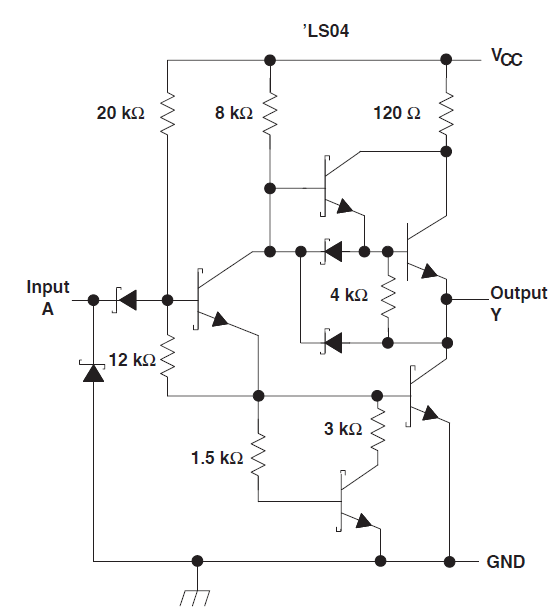
\includegraphics[width=0.5\textwidth]{../grafici/LS04.png}
	\caption{Schema del circuito elettrico di una singola porta appartenente a \code{IC SN74LS04}}
	\label{fig:LS04}
\end{figure}

Il verso delle correnti in input è uscente, infatti con un ingresso \code{HIGH} si hanno correnti nulle, mentre per un valore dell'ingresso corrispondente a \code{LOW} si osserva una corrente uscente dal circuito (vedi \figurename{~\ref{fig:Iin}}, dove le correnti sono però riportate in modulo).

Questo è coerente con quanto atteso dallo circuito elettrico riportato sul datasheet (\figurename{~\ref{fig:LS04}), dove è mostrato che la tensione di almentazione è connessa all'input, per cui, se lasciato flottante, quest'ultimo si trova \code{HIGH}, da cui il naturale comportamento delle correnti (si è verificato misurandolo lo stato dell'input flottante, che risultava effettivamente \code{HIGH}). D'altronde non potrebbe essere diversamente a causa dei diodi a cui è connesso l'input.

\begin{figure}[H]
	\centering
	\includegraphics[width=0.7\textwidth]{../grafici/Iin.pdf}
	\caption{Dati sperimentali relativi alle correnti in ingresso in funzione delle tensioni in ingresso}
	\label{fig:Iin}
\end{figure}

La corrente $I_{IH}$ è nulla, poiché al di sopra di $V_{in} = \unit{1.2}{\volt}$ risultava tale (confronta nota \ref{nota:I0}). La corrente $I_{IL}$ risultava pari a $\unit{210 \pm 10}{\micro\ampere}$ alla tensione $V_{in} = \unit{506 \pm 6}{\milli\volt}$, prossima a quella a cui è riportato il valore del datasheet, mentre risultava $\unit{260 \pm 10}{\micro\ampere}$ alla tensione $V_{in} = \unit{172 \pm 1}{\milli\volt}$, la minima che è stato possibile raggiungere.

La corrente $I_{IH}$, essendo nulla, è compatibile con il valore massimo da datasheet pari a $\unit{40}{\micro\ampere}$, ed anche $I_{IL}$ risultava essere compatibile, in entrambi i casi considerati sopra, con il valore $\unit{-1.6}{\milli\ampere}$ riportato dal datasheet.

\subparagraph{Fanout} La corrente rilevante per il fanout è la massima corrente assorbita dalla porta (ovviamente questo costituisce una limitazione per il numero di porte di questo tipo pilotabili da un'altra porta).
Dunque la corrente rilevante è la corrente $I_{IL}$, il cui massimo valore misurato è $I_{IL}$ = $\unit{260 \pm 10}{\micro\ampere}$.

%qui la corrente è negativa, quindi sputa anziché tirarsela, ma suppongo valga lo stesso

\paragraph{Correnti in uscita} Per misurare le correnti in uscita si è montato il circuito in \figurename{~\ref{fig:NOTout}}.

\begin{figure}[H]
	\centering
	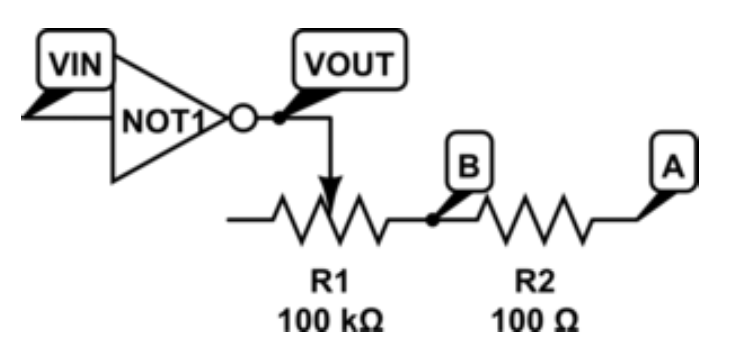
\includegraphics[width=0.5\textwidth]{../grafici/NOTout.png}
	\caption{Schema del circuito usato per la misura delle correnti in uscita dalla porta \code{NOT}}
	\label{fig:NOTout}
\end{figure}

I valori dei componenti usati per la realizzazione del circuito sono riportati in \tablename{~\ref{tab:valori}}. 

\begin{table}[H]
	\centering
	\begin{tabular}{c|c}
		\hline
		$R_1 = \unit{103.0 \pm 0.9}{\kilo\ohm}$ & $R_2 = \unit{99.7 \pm 1.1}{\ohm}$\\
		\hline
	\end{tabular}
	\caption{Valori dei componenti usati per la realizzazione del circuito in esame.}
	\label{tab:valori}
\end{table}

Si è quindi connesso il terminale \code{A} a $V_{in}$ e si è posto quest'ultimo:
\begin{itemize}
	\item a \code{GND}, per misurare $I_{OH}$;
	\item a $V_{cc}$, cioè la tensione di alimentazione, per misurare $I_{OL}$.
\end{itemize}

In entrambi i casi si sono eseguite tre misure: nella prima si sono misurati i valori tipici di corrente di output, corrispondenti a valori tipici di tensione per l'uscita, nelle altre si sono misurate le correnti di output corrispondenti a valori limite di tensione per la logica TTL. \footnote{\href{https://www.allaboutcircuits.com/textbook/digital/chpt-3/logic-signal-voltage-levels/}{https://www.allaboutcircuits.com/textbook/digital/chpt-3/logic-signal-voltage-levels/}}
\footnote{Poiché nella zona intermedia lo stato della porta era instabile si è cercato di andare quanto più possibile vicino ai limiti TTL rimanendo nella zona di stabilità.}

Si è stabilito di misurare le correnti leggendo la tensione ai capi della resistenza $R_2$, cioè la tensione presente tra \code{A} e \code{B}, con il tester digitale. Le misure effettuate sono riportate in \tablename{~\ref{tab:iohiol}}.

\begin{table}[H]
	\centering
	\begin{tabular}{c|c|c|c|c|c|}
		\cline{2-5}
			& \multicolumn{2}{|c|}{Typical values} &	 \multicolumn{2}{|c|}{TTL OUT threshold}\\
		\cline{2-5}
			& $V_{out}$ & $I_{out}$ & $V_{out}$ & $I_{out}$	\\
		\hline
		\multicolumn{1}{|c|}{$I_{OH}$} & $\unit{3.56 \pm 0.03}{\volt}$ & $\unit{106.2 \pm 1.9}{\micro\ampere}$ & $\unit{2.78 \pm 0.02}{\volt}$ &	$\unit{5.81 \pm 0.12}{\milli\ampere}$\\
		\hline
		\multicolumn{1}{|c|}{$I_{OL}$} & $\unit{144 \pm 2}{\milli\volt}$ & $\unit{44.1 \pm 1.3}{\micro\ampere}$ & $\unit{280 \pm 3}{\milli\volt}$ & $\unit{4.01 \pm 0.11}{\milli\ampere}$ \\
		\hline
	\end{tabular}
	\caption{Misure di $I_{OH}$ e $I_{OL}$.}
	\label{tab:iohiol}
\end{table}

Dal datasheet del componente si possono leggere i valori massimi per le correnti misurate, che corrispondono a $I_{OH} = \unit{-0.4}{\milli\ampere}$ e $I_{OL} = \unit{16}{\milli\ampere}$, e dal confronto con i valori in \tablename{~\ref{tab:iohiol}} si ha che nel regime di funzionamento tipico le correnti sono nel range dichiarato dal datasheet, mentre avvicinandosi alla regione di instabilità il valore di $I_{OH}$ supera quello massimo dichiarato, mentre $I_{OL}$ rientra ancora nel margine dato (è da notare però che mentre $I_{OH}$ è misurato quasi a soglia, che corrisponde a $\unit{2.7}{\volt}$, $I_{OL}$ è piuttosto lontano dalla sua), che corrisponde a $\unit{0.5}{\volt}$.

\subparagraph{Variazioni repentine} Si è osservata la presenza di regioni di tensione di output in cui non si riusciva a fissare stabilmente il valore dell'uscita, e la tensione tendeva a portarsi ai margini della regione. Queste regioni (una nella misura di $I_{OH}$ e una in quella di $I_{OL}$) erano instabili proprio perché per variazioni piccole del carico si passava rapidamente da un margine all'altro della regione.
% e se devo dare una spiegazione del perché non la so e quindi mi fermo, amen

\section{Montaggio di Arduino}
Si è montato il circuito impulsatore con il microcontrollore arduino, seguendo le indicazioni riportate sulla scheda. Si è stati attenti a rendere il montaggio più ordinato e compatto possibile al fine di permettere l'utilizzo di altri componenti circuitali sulla basetta. Di seguito è riportato lo schema circuitale del circuito assemblato (\figurename{~\ref{fig:schardu}}). Le resistenze e i condensatori utilizzati sono riportati in \tablename{~\ref{tab:ardu}}. 

\begin{table}[H]
	\centering
	\begin{tabular}{c|c|c|c|c|c|c}
	$R_1 [\Omega$] & $R_2 [\Omega]$ & $R_3 [\Omega]$ & $R_4 [\Omega]$ & Trimmer($R_5 [k \Omega]$) & $C_1 [nF]$ & $C_2 [nF]$\\
	\hline
	974 $\pm$8 & 986$\pm$8 & 990$\pm$8& 990$\pm$8 & 10.3$\pm$0.1 & 107$\pm$4 & 107$\pm$4\\
	\hline
	\end{tabular}
	\caption{Valori delle resistenze e dei condensatori utilizzati per montare arduino e il microcontrollore. I nomi sono riferiti alla \figurename{~\ref{fig:schardu}} .}
	\label{tab:ardu}
\end{table}


\begin{figure}[H]
	\centering
	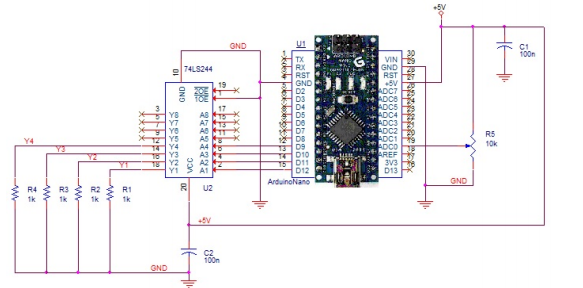
\includegraphics[width=0.5\textwidth]{../grafici/schardu.png}
	\caption{Schema circuito impulsatore con il microcontrollore arduino.}
	\label{fig:schardu}
\end{figure}

Questo circuito genera sui piedini Y1 e Y2 evidenziati in \figurename{~\ref{fig:schardu}}, due onde quadre sfasate di 90$\degree$ con una frequenza variabile tra pochi Hz e 50KHz attraverso il trimmer. Le onde in uscita vengono mostrate in \figurename{~\ref{fig:ardu}} e hanno una frequenza di 859.35$\pm$0.02 Hz.

\begin{figure}[H]
	\centering
	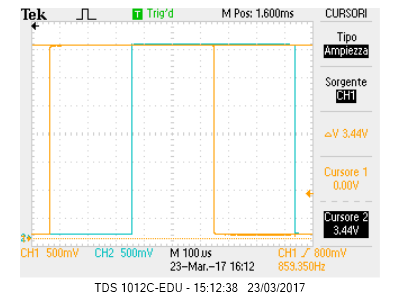
\includegraphics[width=0.5\textwidth]{../grafici/ardu.png}
	\caption{Onde quadre in uscita dai piedini Y1 e Y2 sfasate di 90$\degree$ tra loro.}
	\label{fig:ardu}
\end{figure}


\section{Caratteristiche dinamiche}
Si è inviata in ingresso all'impulsatore un’onda quadra di ampiezza di (4.99$\pm$0.03) V e con la stessa frequenza fissata precedentemente. Al buffer si è poi collegato un circuito NOT. Le onde in ingresso e in uscita al NOT sono mostrate in \figurename{~\ref{fig:notardu}} e, come aspettato, mostrano il corretto funzionamento di questo.

\begin{figure}[H]
	\centering
	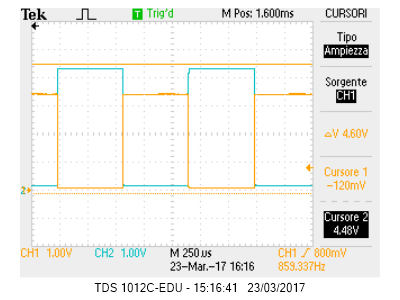
\includegraphics[width=0.5\textwidth]{../grafici/notardu.png}
	\caption{Onde quadre in ingresso e uscita del circuito NOT.}
	\label{fig:notardu}
\end{figure}

\subsection{Misura dei tempi di propagazione}
Si sono misurati i tempi di propagazione del circuito NOT nel passaggio da High(H) a Low(L) e viceversa. Più precisamente, per il passaggio del NOT da H a L si è preso come tempo di propagazione (tPHL) la distanza temporale tra il tempo corrispondente alla metà della differenza di potenziale nel passaggio da L a H all'uscita del buffer e il tempo corrispondente alla metà della differenza di potenziale nel passaggio da H a L del NOT. Allo stesso modo si è proceduto per il calcolo di tPLH dove in tutto ciò che si è scritto sopra basta sostituire H$\leftrightarrow$L. I dati sono riportati in \tablename{~\ref{tab:tprop}} e in \figurename{~\ref{fig:tphlNOT}} è mostrata come esempio la misura di tPHL.

\begin{table}[H]
	\centering
	\begin{tabular}{c|c|c|c|c|c}
	tPHL [ns] & $tPHL_{typ} [ns]$ & $tPHL_{max} [ns]$ & tPLH [ns] & $tPLH_{typ} [ns]$& $tPLH_{max} [ns]$\\
	\hline
	9.4 $\pm$0.4 & 10 & 15 & 15.2$\pm$0.4 & 9 & 15\\
	\hline
	\end{tabular}
	\caption{Misure dei tempi di propagazione tPHL e tPLH del circuito NOT. Sono mostrati anche i valori tipici e massimi forniti sul datasheet.}
	\label{tab:tprop}
\end{table}

\begin{figure}[H]
	\centering
	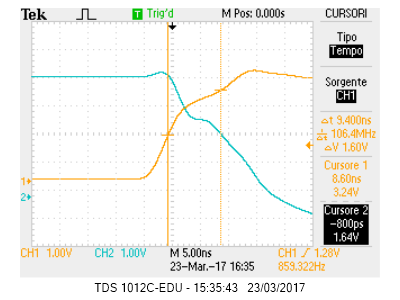
\includegraphics[width=0.5\textwidth]{../grafici/tphlNOT.png}
	\caption{Misura del tempo di propagazione tPHL del circuito NOT mediante l'oscilloscopio.}
	\label{fig:tphlNOT}
\end{figure}

Come si può vedere dalla \tablename{~\ref{tab:tprop}} i valori ottenuti sono compatibili con i valori tipici/massimi riportati sul datasheet del circuito NOT. Gli errori associati a tali misure sono stati calcolati facendo la somma in quadratura dei vari errori riportati sul datasheet dell'oscilloscopio. Inoltre si è trascurato l'errore dovuto alla misura dei valori picco-picco, assumendo pendenza nulla su di essi e quindi trascurandoli nella propagazione.

\subsection{Misura del tempo di salita}
Si sono misurati i tempi di salita e discesa (tra il 10\% e il 90\% dei valori picco-picco) del circuito NOT al suo ingresso (quindi all'uscita del buffer) e alla sua uscita. I dati ottenuti sono riportati in \tablename{~\ref{tab:tsaldisc}}. Nella \figurename{~\ref{fig:temposalita1input}} è mostrata come esempio la misura del tempo di salita all'ingresso del NOT e nella \figurename{~\ref{fig:tempodiscesa}} è mostrata la misura del tempo di discesa all'uscita di esso.

\begin{table}[H]
	\centering
	\begin{tabular}{c|c|c|c}
	$t_{sal,in}$ [ns] & $t_{disc,in}$ [ns] & $t_{sal,out}$ [ns] & $t_{disc,out}$ [ns]\\
	\hline
	12.4$\pm$0.3 & 6.0$\pm$0.3 & 290$\pm$40 &12.8$\pm$0.3\\
	\hline
	\end{tabular}
	\caption{Misure dei tempi di salita e discesa all'ingresso e all'uscita del circuito NOT.}
	\label{tab:tsaldisc}
\end{table}


\begin{figure}[H]
	\centering
	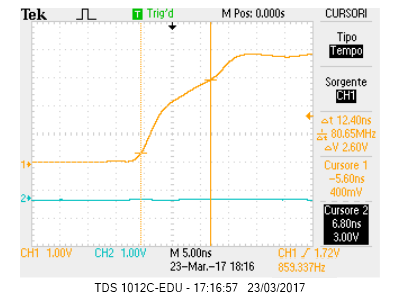
\includegraphics[width=0.5\textwidth]{../grafici/temposalita1input.png}
	\caption{Misura del tempo di salita all'ingresso del NOT.}
	\label{fig:temposalita1input}
\end{figure}

\begin{figure}[H]
	\centering
	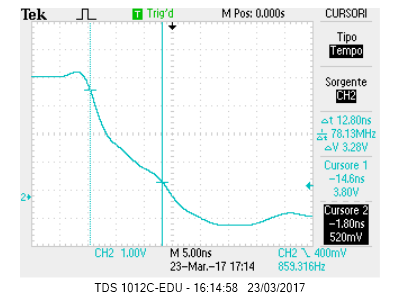
\includegraphics[width=0.5\textwidth]{../grafici/tempodiscesa.png}
	\caption{Misura del tempo di discesa all'uscita del NOT.}
	\label{fig:tempodiscesa}
\end{figure}

Come si può notare dalla \tablename{~\ref{tab:tsaldisc}} il tempo di salita all'uscita del NOT è notevolmente maggiore degli altri tempi di salita e discesa.
Nel misurare questo tempo si è notato che che in realtà erano presenti due fronti, uno molto ripido ("gomito") e uno a bassa pendenza. Come tempo di salita si è scelto di prendere l'intervallo al tra il 10\% e il 90\% della salita complessiva, ma si è riportato per completezza anche il tempo di salita del gomito che risulta essere di 45.6$\pm$ 0.4 ns. L'errore associato alla salita complessiva e la sua misura sono stati stimati a partire dal range di tempi in cui si aveva il 90\% dell'ampiezza picco-picco dell'onda(questo punto ricadeva nella parte di salita a bassa pendenza, perciò si aveva molta più incertezza). Si è presa la distanza temporale tra il 10\% della salita e il più alto valore t in cui si aveva il 90\% dell'ampiezza picco-picco; si è scelta come misura la differenza tra questo tempo e la semiampiezza del range in cui si aveva il 90\% e come errore questa semiampiezza. I due diversi fronti di salita sono mostrati in \figurename{~\ref{fig:temposalita1}}.

\begin{figure}[H]
	\centering
	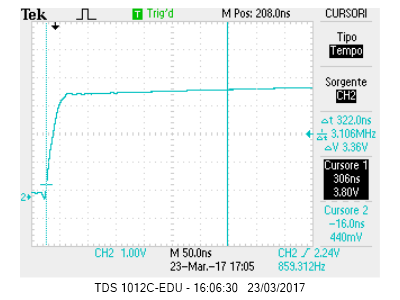
\includegraphics[width=0.5\textwidth]{../grafici/temposalita1.png}
	\caption{Visualizzazione tramite l'oscilloscopio dei due diversi fronti di salita all'uscita del circuito NOT.}
	\label{fig:temposalita1}
\end{figure}

\end{document}